\chapter{Trabalhos Relacionados}
Neste capítulo, são apresentados os trabalhos identificados a partir de uma revisão sistemática da literatura. É importante ressaltar que os trabalhos incluídos aqui representam apenas um extrato da literatura acadêmica, servindo como referencial para o desenvolvimento desta dissertação.
\section{Revisão Sistemática da Literatura}
Esta revisão foca especificamente em abordagens baseadas em IA, particularmente Aprendizado por Reforço (RL) e Aprendizado Profundo (DL), em vez de oferecer uma análise ampla dos métodos tradicionais. Esse foco é motivado pelo crescente consenso na literatura de que as técnicas de IA são essenciais para superar as limitações das abordagens convencionais na adaptação a ambientes complexos e dinâmicos. Os VANTs modernos agora são equipados com processadores poderosos e sensores avançados, permitindo tomada de decisão em tempo real e ajustes dinâmicos às mudanças ambientais. Os objetivos que esta revisão busca enfatizar são:  %Métodos tradicionais, como técnicas baseadas em regras ou otimização estática, frequentemente carecem da flexibilidade necessária para lidar com mudanças imprevisíveis ou condições não estruturadas.

%Avanços recentes nos algoritmos de RL e DL, aliados a melhorias significativas nas capacidades computacionais e sensoriais embarcadas em VANTs, reforçaram ainda mais o potencial transformador das abordagens baseadas em IA. Os VANTs modernos agora são equipados com processadores poderosos e sensores avançados, permitindo tomada de decisão em tempo real e ajustes dinâmicos às mudanças ambientais. Essas capacidades aprimoradas possibilitam que os métodos baseados em IA alcancem níveis superiores de adaptabilidade, escalabilidade e robustez em diversos cenários operacionais. Ao concentrar-se nessas metodologias avançadas, esta revisão busca fornecer insights práticos sobre como a IA pode aprimorar o desempenho de enxames de VANTs, tanto em ambientes reais quanto em simulações de alta fidelidade, abordando desafios que as técnicas tradicionais não conseguem superar de forma eficaz.

\begin{itemize}
    \item \textbf{Validação em Ambientes Reais e Simulações de Alta Fidelidade}: Destacando métodos testados em enxames de VANTs físicos ou simuladores 3D avançados para fornecer insights práticos sobre sua viabilidade.
    \item \textbf{Contribuições Específicas para Tarefas}: Detalhando como os métodos de RL e DL abordam tarefas essenciais do enxame, como planejamento de trajetória, prevenção de colisões e controle de formação em ambientes reais ou simulados.
    \item \textbf{Métricas de Desempenho e Trade-Offs}: Avaliando escalabilidade, eficiência energética e robustez, além de identificar compromissos e desafios na implementação de sistemas de enxame baseados em IA.
\end{itemize}
 
\section{Questões da RSL}
Os questionamentos que guiaram a RSL foram:
\begin{enumerate}
    \item \textbf{RQ1}: Como as abordagens de aprendizado por reforço (RL) e aprendizado profundo (DL) podem lidar com os desafios de escalabilidade, adaptabilidade e robustez em sistemas de enxame de VANTs?

    \item \textbf{RQ2}: Quais são os algoritmos de RL e DL mais avançados utilizados em sistemas de enxame de VANTs?

    \item \textbf{RQ3}: Quais são as contribuições específicas de RL e DL para tarefas de enxame de VANTs, como planejamento de trajetória, prevenção de obstáculos e controle de formação?

    \item \textbf{RQ4}: Quais métricas de desempenho são comumente utilizadas para avaliar sistemas de enxame de VANTs?

    \item \textbf{RQ5}: Como as abordagens de RL e DL melhoram a eficiência energética, a taxa de sucesso das missões e a adaptabilidade em sistemas de enxame de VANTs?

    \item \textbf{RQ6}: Até que ponto os métodos de RL e DL são validados em cenários reais de enxames de VANTs e quais são os desafios para reduzir a lacuna entre simulação e implementação?
\end{enumerate}
 
\section{Metodologia}
 O processo de busca para esta revisão sistemática foi orientado pelo framework PICO (População, Intervenção, Comparação, Resultado), uma metodologia amplamente estabelecida e utilizada em revisões sistemáticas para desenvolver estratégias de busca abrangentes e focadas. O framework PICO facilitou a criação de uma string de busca projetada para capturar os estudos mais relevantes na área de sistemas de enxame de VANTs baseados em IA.

 \begin{table}[ht]
\centering
\caption{Construção da string de busca utilizando o framework PICO}
\begin{tabularx}{\columnwidth}{|c|c|X|}
\hline
\textbf{Letra} & \textbf{Componente} & \textbf{Termos buscados} \\ \hline
P              & Population          & “Multi UAV”, “autonomous drones”, “UAV Swarm”, “unmanned aerial vehicle swarm”, “autonomous UAV” \\ \hline
I              & Intervention        & “multi-agent reinforcement learning”, “Deep Reinforcement Learning”, “Reinforcement learning”, “Deep Learning”, “neural networks”, “MARL”, “DRL” \\ \hline
C              & Comparison          & “exploration”, “avoidance”, “planning”, “formation”, “coordination” \\ \hline
O              & Outcome             & “performance”, “efficiency”, “adaptability”, “robustness”, “scalability” \\ \hline
\end{tabularx}
\label{tab:pico_table}
\end{table}

\subsection{Base de Dados e Resultados}
Para garantir uma coleta abrangente e focada de literatura relevante para esta revisão sistemática, foram utilizadas duas bases de dados acadêmicas renomadas, \textbf{Scopus} e \textbf{IEEE Xplore}. Essas bases foram selecionadas devido à sua ampla cobertura de publicações de alta qualidade nas áreas de robótica, inteligência artificial e sistemas de VANTs.

\subsection{Definição dos Critérios}
Para garantir a seleção dos estudos mais relevantes para as questões de pesquisa e os objetivos desta revisão, um conjunto de critérios de exclusão foi definido e aplicado sistematicamente durante o processo de triagem. Esses critérios foram elaborados para filtrar estudos que não apresentem relevância, rigor metodológico ou alinhamento com o foco principal da revisão. Abaixo estão as principais razões para cada critério:

\begin{itemize}
    \item \textbf{Exclusões Baseadas no Escopo}: Estudos que não abordam enxames de VANTs (por exemplo, sistemas de um único VANT, robôs terrestres) foram excluídos para garantir que a revisão permaneça alinhada com o tema específico da inteligência de enxames de VANTs. Artigos não relacionados à inteligência artificial ou que não discutem técnicas de IA, como aprendizado por reforço (RL) ou aprendizado profundo (DL), foram excluídos, uma vez que a revisão enfatiza o papel da IA no controle de enxames de VANTs.
    
    \item \textbf{Exclusões Baseadas no PICO}: Artigos que não abordam os resultados pretendidos (por exemplo, adaptabilidade, robustez ou escalabilidade) foram excluídos para manter a relevância com os objetivos da pesquisa.
    
    \item \textbf{Exclusões Baseadas na Metodologia}: Estudos com metodologias vagas ou incompletas, como ausência de detalhes sobre algoritmos, simulações ou configurações experimentais, foram excluídos para garantir a inclusão de pesquisas reproduzíveis e confiáveis. Artigos não revisados por pares foram excluídos, a menos que fossem pré-prints relevantes de repositórios renomados, como o arXiv, garantindo o rigor científico dos estudos incluídos.
    
    \item \textbf{Exclusões Baseadas na Aplicação}: Artigos focados em aplicações ou tarefas fora do escopo do comportamento de enxames de VANTs (por exemplo, aplicações industriais, formações de robôs terrestres) foram excluídos. Estudos que não demonstram resultados de simulação em um ambiente 3D ou que não apresentam validação experimental foram excluídos, pois esses aspectos são essenciais para avaliar a aplicabilidade no mundo real e a escalabilidade das abordagens analisadas.
\end{itemize}


O diagrama ilustrado na figura \ref{fig:prisma} resume o processo de seleção dos trabalhos.
\begin{figure}[h]
\centering
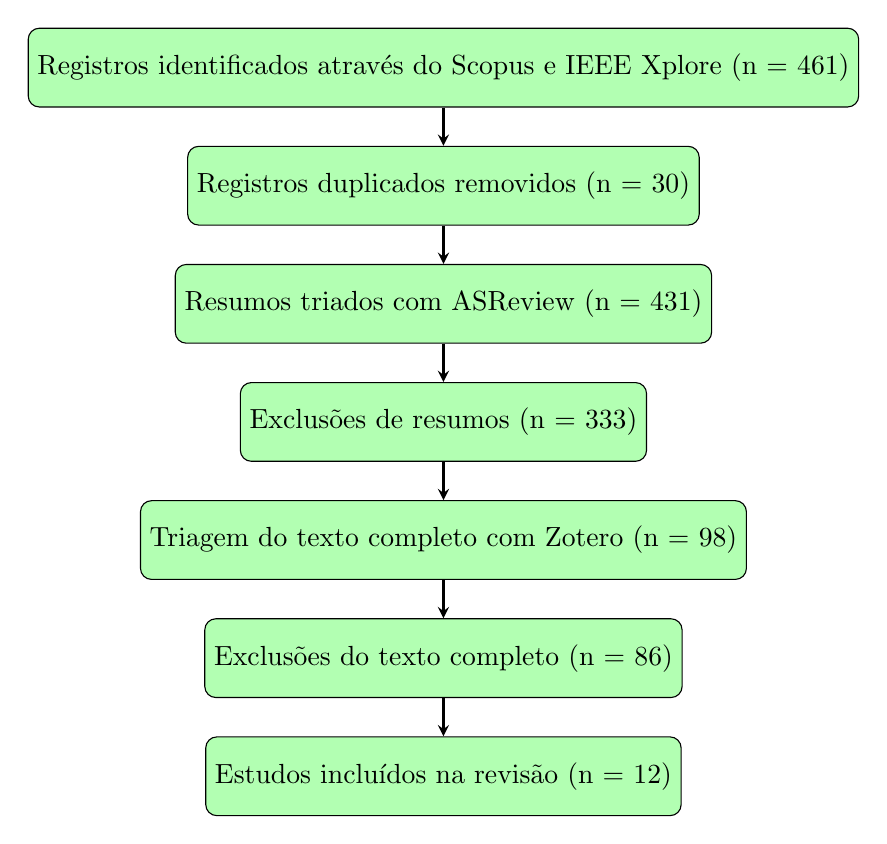
\begin{tikzpicture}[node distance=1.5cm] % Adjusted node distance for vertical spacing

% Define styles
\tikzstyle{process} = [rectangle, rounded corners, minimum width=2cm, minimum height=1cm, text centered, draw=black, fill=green!30]
\tikzstyle{arrow} = [thick,->,>=stealth]

% Nodes
\node (id) [process] {Registros identificados através do Scopus e IEEE Xplore (n = 461)};
\node (duplicates) [process, below of=id] {Registros duplicados removidos (n = 30)};
\node (screen1) [process, below of=duplicates] {Resumos triados com ASReview (n = 431)};
\node (exclude1) [process, below of=screen1] {Exclusões de resumos (n = 333)};
\node (screen2) [process, below of=exclude1] {Triagem do texto completo com Zotero (n = 98)};
\node (exclude2) [process, below of=screen2] {Exclusões do texto completo (n = 86)};
\node (include) [process, below of=exclude2] {Estudos incluídos na revisão (n = 12)};
% Arrows
\draw [arrow] (id) -- (duplicates);
\draw [arrow] (duplicates) -- (screen1);
\draw [arrow] (screen1) -- (exclude1);
\draw [arrow] (exclude1) -- (screen2);
\draw [arrow] (screen2) -- (exclude2);
\draw [arrow] (exclude2) -- (include);

\end{tikzpicture}
\caption{Fluxograma PRISMA ilustrando o processo de revisão sistemática}
\label{fig:prisma}
\end{figure}

\section{Resultados}
Os artigos selecionados destacam coletivamente o papel transformador das técnicas de Aprendizado por Reforço (RL) e Aprendizado Profundo (DL) no avanço das capacidades dos sistemas de enxame de VANTs. Por fim a tabela \ref{tab:swarm_summary} resume as informações dos trabalhos considerados.
\clearpage


%Tabela desajustada, arrumar
%\subsection{Resumo dos Trabalhos}
\begin{table*}[p]
\centering
\caption{Resumo dos trabalhos considerados pela revisão}
\renewcommand{\arraystretch}{1} % Adjust row height for vertical spreading
\setlength{\tabcolsep}{4pt} % Adjust column spacing
\resizebox{1\textwidth}{!}{
\begin{tabular}{|p{6cm}|p{4cm}|p{3cm}|p{3cm}|}
\hline
\textbf{Contribuição} & \textbf{Algoritmos} & \textbf{Arquitetura} & \textbf{Tarefa} \\ \hline
Dynamic formation control using DRL under operational uncertainty \cite{ID1}. & Proximal Policy Optimization (PPO), Deep Deterministic Policy Gradient (DDPG) & Centralized & Formation control, collision avoidance \\ \hline
Multi-agent PPO for combat UAV decision-making with reduced oscillation and enhanced stability \cite{ID2}. & Multi-Agent PPO & Centralized & Maneuvering decision-making \\ \hline
Distributed area coverage using FDSAC with centralized training and decentralized execution \cite{ID3}. & Fully Decentralized Soft Actor-Critic (FDSAC) & Decentralized & Dynamic area coverage \\ \hline
Multi-agent DRL for coverage-aware task allocation combining UAV and human collaboration \cite{ID4}. & Multi-Agent Actor-Critic (MAAC) & Decentralized & Task allocation, coverage optimization \\ \hline
Multi-drone shepherding for flock management using MTDDPG \cite{ID5}. & Multi-Task Deep Deterministic Policy Gradient (MTDDPG) & Decentralized & Shepherding, collision avoidance \\ \hline
MARL with adversarial randomization for robustness in dynamic environments \cite{ID6}. & Adversarial Domain Randomization with PPO & Decentralized & Dynamic task allocation, collision avoidance \\ \hline
Two-stage DRL for efficient target tracking with expert-guided exploration \cite{ID7}. & Double Deep Q-Network (DDQN), Expert-Guided Exploration & Decentralized & Target tracking \\ \hline
CBC-TP Net for UAV pursuit-evasion games in complex urban settings \cite{ID8}. & Cross-Boundary Cooperative Task-Planning Net (CBC-TP Net) & Decentralized & Pursuit-evasion \\ \hline
Vision-based formation control using YOLOv7 and DeepSORT in GNSS-denied environments \cite{ID9}. & YOLOv7, DeepSORT & Hybrid Hierarchical & Formation control \\ \hline
PPO with RNN layers for path planning in partially observable environments \cite{ID10}. & PPO with Recurrent Neural Network (RNN) layers & Decentralized & Path planning, collision avoidance \\ \hline
IPBO framework for multitarget tracking using island-based decentralized policy optimization \cite{ID11}. & Island Policy-Based Optimization (IPBO) & Decentralized & Multitarget tracking \\ \hline
Belief-policy interrelation framework using GAIL for coordination in heterogeneous swarms \cite{ID12}. & Generative Adversarial Imitation Learning (GAIL) & Decentralized & Coordination, formation control \\ \hline
\end{tabular}
}
\label{tab:swarm_summary}
\end{table*}




\clearpage



\subsection{Aprimoramento na Execução de Tarefas}
\subsubsection{Controle Dinâmico de Formação}
Vários artigos, incluindo \cite{ID1}, demonstram a integração de algoritmos de RL e DL para permitir que enxames de VANTs mantenham formações sinérgicas em ambientes incertos. Por exemplo, o framework P-DRL em \cite{ID1}, utilizando algoritmos como A3C e DQN, aborda a incerteza operacional ao dividir o problema de controle em subproblemas mais simples, reduzindo significativamente a complexidade computacional, enquanto mantém a capacidade de resposta em tempo real. No entanto, limitações na prevenção de colisões indicam que melhorias adicionais na interação entre múltiplos agentes são necessárias.

\subsubsection{Manobras e Rastreamento de Múltiplos Alvos}
Os artigos \cite{ID2} e \cite{ID11} enfrentam os desafios da tomada de decisão cooperativa e do rastreamento de múltiplos alvos em ambientes 3D dinâmicos. Utilizando métodos avançados de MARL, como MP3O e frameworks otimizados por recompensa, esses trabalhos alcançam melhorias notáveis na eficiência da tomada de decisão e na versatilidade do enxame. Além disso, o conceito de enxame dinâmico em \cite{ID11} oferece soluções inovadoras para particionamento e reagrupamento de VANTs com base na distribuição de alvos, aumentando a flexibilidade operacional.

\subsubsection{Alocação de Tarefas e Cobertura de Área}
A alocação de tarefas e a cobertura de área emergem como áreas de foco críticas em \cite{ID4} e \cite{ID3}. Os algoritmos baseados em DRL propostos distribuem de forma eficiente as tarefas de sensoriamento e ajustam dinamicamente os pontos de cobertura. Por exemplo, o método de alocação de tarefas Pareto-ótimo em \cite{ID4} combina a colaboração entre VANTs e humanos, enfatizando aplicações no mundo real, como cidades inteligentes e serviços públicos. Esses estudos ressaltam o potencial das técnicas de DL na otimização do desempenho das tarefas, ao mesmo tempo em que lidam com restrições como comunicação e poder computacional.

\subsubsection{Prevenção de Colisões e Navegação}
Técnicas como as descritas em \cite{ID7} e \cite{ID11} priorizam a navegação segura e a prevenção de obstáculos por meio de mecanismos avançados de recompensa e frameworks de treinamento com RL. A abordagem DRL em duas etapas apresentada em \cite{ID7}, incorporando experiência de especialistas, melhora a velocidade de convergência e a capacidade de generalização em ambientes dinâmicos. Isso reduz os custos de treinamento, garantindo uma navegação confiável para múltiplos agentes.


\subsection{Melhorias de Desempenho e Trade-Offs}
\subsubsection{Escalabilidade}
A escalabilidade, um desafio crítico em sistemas de enxame de VANTs, foi abordada de forma eficaz em diversos estudos. Por exemplo, o framework P-DRL em \cite{ID1} demonstrou controle de formação em tempo real para enxames compostos por 10–20 VANTs, ampliando significativamente a escalabilidade da coordenação multiagente. Da mesma forma, \cite{ID11} introduziu um conceito de enxame dinâmico que permitiu a partição e reagrupamento de grupos de VANTs de forma adaptativa, garantindo flexibilidade para atender às mudanças nos requisitos das tarefas. Essas abordagens ressaltam o potencial dos métodos de RL na expansão das operações do enxame sem comprometer o desempenho, embora frequentemente exijam recursos computacionais substanciais durante o treinamento.

\subsubsection{Tempo de Execução}
A redução do tempo de execução para tarefas como planejamento dinâmico de trajetória e controle de formação é essencial para aplicações em tempo real. Estudos como \cite{ID5} utilizaram aprendizado por reforço profundo multitarefa (MT-DDPG) para acelerar a conclusão de operações de pastoreio. Da mesma forma, \cite{ID9} empregou modelos leves de DL, como o YOLOv7, para realizar controle de formação baseado em visão em tempo real, demonstrando tempos de execução adequados para processamento embarcado. No entanto, essas melhorias aumentam a complexidade algorítmica e exigem treinamento intensivo em recursos computacionais.

\subsubsection{Taxa de Sucesso}
O aprimoramento da taxa de sucesso em tarefas do enxame, como prevenção de colisões e alocação dinâmica de tarefas, foi um foco central. Por exemplo, \cite{ID2} relatou maior estabilidade e eficiência na tomada de decisão cooperativa utilizando o algoritmo MP3O, melhorando as taxas de sucesso em manobras de combate aéreo. Além disso, \cite{ID7} demonstrou que o pré-treinamento de agentes com dados especializados levou a uma convergência mais rápida e a resultados de rastreamento mais confiáveis, especialmente em ambientes com obstáculos. No entanto, esses sucessos geralmente dependem de um design cuidadoso das funções de recompensa e otimizações específicas do domínio, o que pode limitar a generalização dos métodos.

\subsubsection{Resiliência}
A resiliência a incertezas ambientais e falhas do sistema foi destacada em estudos que empregam técnicas de randomização de domínio. \cite{ID6} propôs a randomização adversarial de domínio para melhorar a robustez das políticas MARL na transição de simulação para realidade, garantindo desempenho consistente em diversos cenários operacionais. Da mesma forma, \cite{ID8} introduziu um framework de perseguição e evasão que manteve o sucesso da missão mesmo quando alguns VANTs do enxame foram comprometidos. Embora esses métodos aumentem a resiliência, geralmente exigem alto custo computacional e ambientes de simulação extensivos para um treinamento eficaz.

\subsubsection{Trade-Offs}
\begin{itemize}
    \item \textbf{Demandas Computacionais}: Métodos como randomização adversarial de domínio \cite{ID6} e frameworks hierárquicos profundos \cite{ID8} exigem altos recursos computacionais, o que pode limitar sua implementação em sistemas de VANTs com restrições de hardware.
    \item \textbf{Complexidade do Treinamento}: Técnicas que enfatizam adaptabilidade e resiliência, como reconfiguração dinâmica de enxame \cite{ID11} ou DRL em duas etapas \cite{ID7}, frequentemente envolvem pipelines de treinamento complexos, demandando expertise significativa e tempo de desenvolvimento.
    \item \textbf{Implantação no Mundo Real}: Embora os resultados em simulação sejam promissores, métodos como P-DRL \cite{ID1} e MP3O \cite{ID2} enfrentam desafios na transição para aplicações reais devido a fatores como imprecisões nos sensores e restrições de comunicação.
\end{itemize}



\section{Discussão}
\subsection{Principais Descobertas}
Esta revisão sistemática explorou as contribuições das técnicas de Aprendizado por Reforço (RL) e Aprendizado Profundo (DL) para o avanço dos sistemas de enxame de VANTs, destacando seu potencial transformador na solução de desafios críticos. Nos artigos revisados, foram alcançadas melhorias significativas em escalabilidade, tempo de execução, taxa de sucesso e resiliência. As principais contribuições incluem:

\begin{itemize}
    \item \textbf{Controle Dinâmico de Formação}: Estudos como \cite{ID1} demonstraram frameworks capazes de realizar controle de formação em tempo real para enxames de VANTs de médio porte, reduzindo a complexidade computacional por meio de algoritmos avançados de RL, como A3C e DQN.
    \item \textbf{Tomada de Decisão Multiagente e Rastreamento}: Abordagens inovadoras, como MP3O (\cite{ID2}) e conceitos de enxame dinâmico (\cite{ID11}), aprimoraram significativamente a tomada de decisão cooperativa e o rastreamento de múltiplos alvos, melhorando a eficiência operacional e a adaptabilidade.
    \item \textbf{Alocação de Tarefas e Cobertura de Área}: Métodos como alocação de tarefas Pareto-ótima (\cite{ID4}) e cobertura baseada em FDSAC (\cite{ID3}) apresentaram técnicas eficazes para equilibrar a distribuição da carga de trabalho e otimizar a eficiência do sensoriamento, mesmo em ambientes com restrições de comunicação.
    \item \textbf{Prevenção de Colisões e Navegação}: Frameworks como os descritos em \cite{ID7} e \cite{ID6} forneceram soluções robustas para navegação em ambientes complexos, com avanços em modelagem de recompensas e randomização de domínio, garantindo operações livres de colisões e melhores transições entre simulação e realidade.
    \item \textbf{Validações em Ambientes Reais}: Alguns estudos (\cite{ID5}, \cite{ID9}) validaram seus métodos em cenários reais, demonstrando viabilidade prática e oferecendo uma base para melhorias futuras.
\end{itemize}

\subsection{Lacunas e Desafios Não Resolvidos}
Apesar desses avanços, diversas lacunas permanecem, apontando para oportunidades de pesquisa futura:
\begin{enumerate}
    \item \textbf{Escalabilidade para Enxames Maiores}: Embora muitos métodos tenham melhorado a coordenação em enxames de médio porte (por exemplo, 10–20 VANTs em \cite{ID1}), a escalabilidade para enxames maiores ainda é um desafio aberto. São necessários algoritmos eficientes que possam escalar sem um aumento proporcional na complexidade computacional.
    \item \textbf{Redução da Lacuna entre Simulação e Realidade}: Embora métodos de randomização de domínio (\cite{ID6}) tenham mostrado potencial, a tradução dos resultados simulados para operações no mundo real é limitada por ruído nos sensores, variabilidade ambiental e restrições do sistema. Melhorar a robustez em aplicações reais continua sendo essencial.
    \item \textbf{Eficiência Energética e Otimização de Recursos}: Embora alguns estudos tenham abordado o consumo de energia indiretamente, estratégias dedicadas para otimizar o uso energético em todo o enxame ainda são pouco exploradas.
    \item \textbf{Métricas Padronizadas e Benchmarking}: A ausência de métricas padronizadas entre os estudos (\cite{ID3}, \cite{ID4}) dificulta comparações diretas. O estabelecimento de um framework unificado de benchmarking facilitaria avaliações consistentes do desempenho dos enxames.
    \item \textbf{Integração de Sistemas Heterogêneos}: Estudos como \cite{ID12} introduziram esforços iniciais para a coordenação de enxames heterogêneos, mas são necessárias investigações mais aprofundadas sobre o equilíbrio das disparidades de recursos e a alocação de tarefas entre diferentes tipos de VANTs.
\end{enumerate}

\section{Comparação com Estado da Arte}
A tabela \ref{tab:marl_comparison} ilustra como o trabalho proposto se posiciona em relação aos trabalhos da revisão de literatura. Os critérios adotados na comparação foram:
\begin{itemize}
    \item Execução Descentralizada (DE): Verifica se a abordagem adotada pelo trabalho possibilita execução descentralizada pelos agentes, isto é, se o enxame não necessita de um nó central que envia os comandos para execução.
    
    \item Escalabilidade (Scalable): Verifica se a abordagem de controle do enxame permite a quantidade de agentes pode aumentar sem afetar o desempenho.
    
    \item Coordenação (Coord): Se há coordenação entre as ações dos agentes no ambiente que executam a missão.
    
    \item Espaço de Ação Contínuo (Cont): Verifica se o domínio do espaço de ações dos agente é contínuo ou discreto.
    
    \item Visão Computacional (Vision): Se a abordagem utiliza algum tipo de informação visual capturada pelos agentes em seu espaço de observações do algoritmo.
    
    \item Comunicação (Comm): Se há troca de informações entre os agentes através de algum meio de comunição.
    
    \item Missão Global (GM): Se a missão do enxame envolve tarefas complexas além das tarefas atividades comuns, como por exemplo: rastreamento de alvos, transporte de carga, cobertura de área e reconstrução 3D.
    
    \item Planejamento de Caminho (PP): Se o trabalho lida com a atividade de planejamento de trajetória.
    
    \item Prevenção de Colisões (CA): Se o trabalho aborda a atividade de prevenção de colisões.
    
    \item Controle de Formação (FC): Se o trabalho aborda a atividade do controle de formação do enxame.
\end{itemize}

\paragraph{Ajustar tabela para o CAP 5 secao de comparacao com SOTA}
\begin{table}[h]
\centering
\caption{Quadro comparativo da proposta com estado da arte.}
\label{tab:marl_comparison}
\begin{adjustbox}{width=\textwidth}
\begin{tabular}{ccccccccccc}
\toprule
  Trabalho &DE&Scalable&Coord&Cont&Vision&Comm&GM&PP&CA&FC \\
  
\midrule
  \cite{ID1} &  \xmark & \cmark & \cmark & \cmark & \xmark & \cmark & \xmark & \cmark & \cmark &\cmark  \\
  \cite{ID2} &  \cmark & \xmark & \xmark & \cmark & \xmark & \xmark & \cmark & \cmark & \xmark &\xmark \\
  \cite{ID3} &  \cmark & - & \xmark & \xmark & \xmark & \cmark & \cmark & \xmark & \cmark & \xmark  \\
  \cite{ID4} &  \cmark & \xmark & \cmark & \xmark & \xmark & \xmark & \cmark & \cmark & \cmark & \xmark\\
  \cite{ID5} &  \cmark & \xmark & \cmark & \cmark & \xmark & \xmark & \cmark & \cmark & \xmark & \cmark \\
  \cite{ID6} &  \cmark & \xmark & \cmark & \cmark & \cmark & - & \cmark & \cmark & \xmark & \cmark \\
  \cite{ID7} &  \cmark & \xmark & \cmark & \cmark & \cmark & \xmark & \cmark & \cmark & \cmark & \xmark \\
  \cite{ID8} &  \cmark & \xmark & \cmark & \cmark & \xmark & \cmark & \cmark & \cmark & \cmark & \xmark \\
  \cite{ID9} &  \xmark & \xmark & \cmark & \cmark & \cmark & \cmark & \xmark & \xmark & \xmark & \cmark \\
  \cite{ID10} &  \cmark & \xmark & \xmark & \cmark & \xmark & \cmark & \xmark & \cmark & \cmark & \xmark \\
  \cite{ID11} &  \cmark & \cmark & \cmark & \xmark & \xmark & \xmark & \cmark & \cmark & \cmark & \cmark \\
  \cite{ID12} &  \cmark & \xmark & \cmark & \cmark & \xmark & \xmark & \xmark & \xmark & \xmark & \cmark  \\
  Proposta &  \cmark & \cmark & \cmark & - & \cmark & \cmark & \cmark & \cmark & \cmark &\cmark  \\
\bottomrule
\end{tabular}
\end{adjustbox}
\end{table}

% \section{Atualização do Estado da Arte Assistida por Ferramentas de IA}

% Com o objetivo de atualizar o estado da arte e incorporar trabalhos recentes publicados após a condução da revisão sistemática formal, foi realizada uma etapa complementar de busca bibliográfica assistida por ferramentas de inteligência artificial. Nesta etapa, utilizou-se um mecanismo de busca baseado em modelos de linguagem de grande porte, configurado para consultar bases acadêmicas consolidadas, como IEEE Xplore, Elsevier e arXiv.

% As consultas foram estruturadas a partir das mesmas questões de pesquisa (RQ1–RQ6) e dos termos definidos no framework PICO, garantindo consistência metodológica com a revisão sistemática original. Os resultados retornados foram submetidos a uma curadoria manual rigorosa, incluindo leitura de títulos, resumos e, quando pertinente, do texto completo, bem como aplicação dos mesmos critérios de inclusão e exclusão previamente definidos.

% É importante destacar que a ferramenta de IA foi utilizada exclusivamente como um meio de apoio à identificação de estudos relevantes, não substituindo o julgamento crítico do pesquisador nem os procedimentos formais de seleção e análise dos trabalhos incluídos nesta dissertação.
